% This document is available under the Creative Commons Attribution-ShareAlike
% License; additional terms may apply. See
%   * http://creativecommons.org/licenses/by-sa/3.0/
%   * http://creativecommons.org/licenses/by-sa/3.0/legalcode
%
% Copyright 2010 Jérôme Pouiller <jezz@sysmic.org>
%

\part{Fabriquer}

{
\setbeamertemplate{background canvas}{}
\begin{frame}[plain]
  \partpage
  \begin{textblock}{10}(6,12)
    %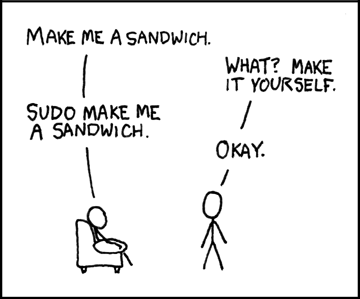
\includegraphics[height=30mm,width=30mm]{sandwich}
    \begin{quote}
      \rmfamily\textit\textbf\color{darkgray}{\large
        ``Talk is cheap. Show me the code.''}
        \vskip3mm\hspace*\fill{\small--- Torvalds, Linus (2000-08-25). Message to linux-kernel mailing list}
    \end{quote}
  \end{textblock}
\end{frame}
}

\begin{frame}
  \tableofcontents
\end{frame}

\section{Compilation des differents éléments}

\subsection{Compilation du noyau}

\begin{frame}[fragile=singleslide]{Récupération des sources}
  Où récupérer les sources du noyau?
  \begin{enumerate}
  \item Utiliser  les sources souvent fournies.  Il arrive souvent
    qu'elles  contiennent  des  drivers particuliers  et  qu'elles
    soient déjà configurées
  \item Utiliser \cmd{git clone} (nous y reviendrons)
  \item Télecharger sur \file{kernel.org}
  \end{enumerate}
  \note[item]{Fonctionne aussi avec 2.6.37}
  \begin{lstlisting}
host$ wget http://www.kernel.org/pub/linux/kernel/v3.X/linux-3.10.32.tar.bz2
host$ tar xvjf linux-3.10.32.tar.bz2
  \end{lstlisting}
\end{frame}

\begin{frame}[fragile=singleslide]{Interface de configuration du noyau}
  \begin{itemize}
    \item Utilise Kconfig
      \begin{lstlisting}
host$ make help
host$ mkdir build
host$ make O=build ARCH=arm CROSS_COMPILE=arm-linux- menuconfig
       \end{lstlisting}
     \item  Beaucoup d'options,  mais il  y a  l'aide (\verb+<h>+)  et la
       recherche (\verb+</>+)
    \item La configuration est sauvée dans \file{.config}
    \item    \verb+at91sam9263_defconfig+   permet   de    charger   une
      configuration pré-établie pour notre carte
      \begin{lstlisting}
host$ make O=build ARCH=arm CROSS_COMPILE=arm-linux- at91sam9263_defconfig
      \end{lstlisting}
    \begin{itemize}
    \item Certains constructeur vous  fournirons un patch ajoutant une
      cible \verb+_defconfig+
    \item D'autres vous fournirons un \file{.config}
    \end{itemize}
  \end{itemize}
\end{frame}

\begin{frame}[fragile=singleslide]{Compilation du noyau}
  \begin{itemize}
  \item Vérifier les options du type de processeur
  \item Cocher NFS
  \item Le reste ne devrait pas empêcher de démarrer votre cible
  \item La compilation se lance avec
    \begin{lstlisting}
host$ make O=build ARCH=arm CROSS_COMPILE=arm-linux- XXImage
    \end{lstlisting}
  \item \verb+XX+ fait référence au format de la binaire produite:
    \begin{itemize}
    \item Le premier octet est-il du code?
    \item Respecte-t-il le format ELF?
    \item Y a-t-il un format particulier d'entête à respecter ?
    \end{itemize}
  \item Dans  le doute,  il faut consulter  la documentation  de votre
    bootloader
  \end{itemize}
\end{frame}

\begin{frame}[fragile=singleslide]{Compiler le noyau}
  Dans notre cas, nous utilisons U-Boot (standard)
  \begin{itemize}
  \item Compilation
    \begin{lstlisting}
host% apt-get install u-boot-tools
host$ make O=build ARCH=arm CROSS_COMPILE=arm-linux- uImage
    \end{lstlisting}
  \item Partage de l'image par TFTP
    \begin{lstlisting}
host% cp build/arch/arm/boot/uImage /var/lib/tftpboot/
    \end{lstlisting} % $ 
    \note[item]{C'est mieux de compiler avec -j3}
    \note[item]{Il faut les laisser démarrer en NFS}
  \end{itemize}
  \note{Parler de l'installation des modules et de l'option INSTALL\_MOD\_PATH}
\end{frame}

\begin{frame}[fragile=singleslide]{Compilation du noyau}
  Fichiers produits (ou productibles) par la compilation:
  \begin{itemize}
  \item  \verb+vmlinux+:  L'image  ELF  du  noyau.   Lisible  par  les
    debugueurs, certains flasheurs, certains bootloaders
  \item  \verb+Image+:  \verb+vmlinux+   strippé  et  préfixé  par  un
    mini-bootloader   permettant    de   sauter   sur    la   fonction
    \verb+start_kernel+ de \verb+vmlinux+.
  \item  \verb+bzImage+  et   \verb+zImage+: Comme \verb+Image+ mais compressé en \cmd{bz2} ou \cmd{gz}.
  \item  \verb+vmlinuz+: Normalement  équivalent  du \verb+bzImage+.
    %normalement, il  s'agit de\verb+vmlinux+ compressé  et strippé des
    %informations inutiles  au démarrage. Inutilisable  dans l'état, il
    %est nécessaire de lui adjoindre un bootloader pour le décompresser
    %et l'exécuter.
  \item  \verb+xipImage+  :  Idem  \verb+Image+ mais  destiné  à  être
    exécuté  directement  sur un  \emph{eeprom}  sans  être copier  en
    mémoire au préalable.
  \item  \verb+uImage+:  \verb+zImage+ avec  une  entête spéciale  pour
    \emph{u-boot}.
  \end{itemize}
%   Il est possible  de générer des image au  format SRecord en utiliant
%   \cmd{objcopy}
%   \begin{lstlisting}
% host$ objcopy -O srec vmlinux vmlinux.srec
%    \end{lstlisting}
  \note[item]{Reprendre le  slide de freeelectron très  bien foutu sur
    le sujet}
\end{frame}

\subsection{Création de l'init}

\begin{frame}[fragile=singleslide]{Démarrage du noyau}
  \begin{itemize}
  \item  A  la fin  du  démarrage  du noyau,  celui  donne  la main  à
    l'éxecutable déclaré  avec \verb+init=+. Par défaut,  il s'agit de
    \file{/sbin/init}
  \item \cmd{init} ne se termine jamais
  \item  Les  arguments  nons  utilisés  par le  noyau  sont  passé  à
    \cmd{init}
  \item On peut  estimer que notre système démarre  à partir du moment
    ou nous  obtenons un shell (c'est  en tous cas  la que la
      plupart des intégrateur Linux embarqué s'arreterons)
  \item Du moins complexe au plus complexe à démarrer:
  \begin{itemize}
    \item \verb+init=/hello-arm-static+
    \item \verb+init=/hello-arm+
    \item \verb+init=/bin/sh+
    \item \verb+init=/sbin/init+
    \end{itemize}
  \end{itemize}
  Effectuons ces tests avec le Rootfs original et un Rootfs vierge.
\end{frame}

\begin{frame}[fragile=singleslide]{Démarrer l'espace utilisateur}
  Après le démarrage, le noyau ne trouve pas l'init:
    \begin{lstlisting}
[...]
Kernel panic - not syncing: No init found.  Try passing init= option to kernel.
    \end{lstlisting}

    Copions maintenant  \verb+hello-arm-static+ et \verb+hello-arm+ et
    essayons de démarrer avec.

     \verb+hello-arm-static+ fonctionne, mais pas \verb+hello-arm+
\end{frame}

\begin{frame}[fragile=singleslide]{Installation des bibliothèques de base}
  Les bibliothèques de base  (\cmd{libc} et apparentés) sont forcement
  fournies avec le cross-compilateur, car elles y sont intimement liés
  \begin{itemize}
  \item Liste des bibliothèques nécessaires
    \begin{lstlisting}
host$ arm-linux-ldd --root . hello-arm
    \end{lstlisting}
    \item Copie
    \begin{lstlisting}
host$ mkdir lib
host$ cp /opt/arm-linux-.../lib/ld-uClibc-1.0.9.so lib
host$ cp /opt/arm-linux-.../lib/libuClibc-1.0.9.so lib
    \end{lstlisting}
  \end{itemize}
\end{frame}

\begin{frame}[fragile=singleslide]{Installation des bibliothèques de base}
  \begin{itemize}
  \item Configuration de \cmd{ldconfig}
    \begin{lstlisting}
host$ echo /lib > etc/ld.so.conf
host$ echo /usr/lib >> etc/ld.so.conf
    \end{lstlisting}
  \item Création des liens symboliques
    \begin{lstlisting}
host$ ldconfig -r . -N
    \end{lstlisting}
  \item Création du cache. Le  cache n'est pas obligatoire, mais si il
    existe, il doit être à jour
    \note[item]{Faire un exo sur PC avec ldconfig}
    \begin{lstlisting}
host$ ldconfig -r .
    \end{lstlisting}
  \end{itemize}
  Nous pouvons maintenant démarrer avec \verb+init=/hello-arm+
\end{frame}

\subsection{Compilation de l'espace utilisateur}

\begin{frame}[fragile=singleslide]{Busybox}
  \begin{itemize}
  \item  Contient la plupart  des binaire  nécéssaire pour  démarrer un
    système
  \item Attention, ce ne  sont pas les meme outils que sur  PC. Il y a
    souvent des option non-implémentés ou des comportements différents
  \item Téléchargement
    \begin{lstlisting}
host$ wget http://busybox.net/downloads/busybox-1.23.2.tar.bz2
host$ tar xvjf busybox-1.23.2.tar.bz2
host$ mkdir build
    \end{lstlisting}
  \item On retrouve \cmd{Kconfig}
    \begin{lstlisting}
host$ make O=build CROSS_COMPILE=arm-linux- menuconfig
    \end{lstlisting}
  \end{itemize}
\end{frame}

\begin{frame}[fragile=singleslide]{Busybox}
  \begin{itemize}
  \item On trouve pleins d'outils
    \note[item]{TODO: mettre en plusieurs colonnes}
  \item    Au   minimum,    vérifions les options    \cmd{ash},   \cmd{init},    les
    \emph{Coreutils}
  \item Vérifions le chemin d'installation
    %\cmd{dmesg},   \cmd{ifconfig},   \cmd{mount},
    %\cmd{tftp}, \cmd{tar}, \cmd{reboot}, \cmd{vi}, \cmd{flashcp}
    \note[item]{TODO: mettre en plusieurs colonnes}
  %\item         Et         aussi:        \verb+CONFIG_PLATFORM_LINUX+,
  %  \verb+CONFIG_FEATURE_EDITING+,        \verb+CONFIG_FEATURE_DEVPTS+,
  %  \verb+CONFIG_LONG_OPTS+,                  \verb+CONFIG_SHOW_USAGE+,
  %  \verb+FEATURE_VERBOSE_CP_MESSAGE+, \verb+IOCTL_HEX2STR_ERROR+
  \end{itemize}
  \note[item]{TODO P2 Lister de manière exaustive}
\end{frame}

\begin{frame}[fragile=singleslide]{Installation de Busybox}
  \begin{itemize}
  \item Configurons le chemin de destination vers \file{\~/nfs}
    \begin{lstlisting}
host$ make O=build CROSS_COMPILE=arm-linux-
host$ make O=build CROSS_COMPILE=arm-linux- CONFIG_PREFIX=~/nfs install
    \end{lstlisting}
    \note[item]{Compiler avec -j3}
  \item  L'installation créé  des  liens symboliques  vers la  binaire
    \cmd{busybox}
  \item  Sans  Busybox,  toutes  ces  binaires  seraient  séparées  et
    dispersées sur une dizaine de sources
  \item Nous pouvons maintenant démarrer avec \verb+init=/bin/sh+
    \note[item] {Démarrer avec  console=ttyS0,115200 afin d'éviter les
      problème avec le jobs: Non ca ne marche pas}
  \item \verb+init=/sbin/init+ pose encore quelques problèmes.
  \end{itemize}
\end{frame}

\begin{frame}[fragile=singleslide]{Configuration de \cmd{init}}
  Il est possible de configurer \cmd{init} avec le fichier
  \file{/etc/inittab}
  \begin{itemize}
  \item Lancement automatique d'un shell
    \begin{lstlisting}
host$ echo "::askfirst:/bin/sh" > etc/inittab 
    \end{lstlisting}
  \item Appel d'un script de démarrage.
    \begin{lstlisting}
host$ echo "::sysinit:/etc/init.d/rcS" >> etc/inittab
host$ mkdir etc/init.d
host$ echo "#!/bin/sh" > etc/init.d/rcS
host$ chmod +x etc/init.d/rcS
    \end{lstlisting}
  \end{itemize}
  Documentation disponible sur la page de man \emph{inittab(5)}
  (disponible ici: \url{http://tfm.cz/man/5/inittab}).\\[2ex]
  Des  fichier de  configuration  de init  et  d'autres utilitaire  de
  busybox sont disponibles dans \file{busybox/examples}
  \note[item]{tester  avec console=ttyS0,115200  et retirer  "ttyS0 de
    l'inittab": Non ca ne marche pas}
\end{frame}

\begin{frame}[fragile=singleslide]{Autres \cmd{init}}
  Il existe d'autres formes d'\cmd{init}:
  \begin{itemize}
  \item SystemV (celui que nous utilisons)
  \item runit (aussi proposé par Busybox)
  \item upstart (utilisé autrefois par Ubuntu)
  \item systemd (utilisé par le reste du monde)
  \end{itemize}
  Ces \cmd{init},  plus modernes  offrent de nouvelles  fonctionnalités et
  plus de robustesse pour le système.
\end{frame}

\begin{frame}[fragile=singleslide]{Compilons init}{Fichiers de configuration}
  Nous  pouvons  maintenant  démarrer avec  \cmd{init=/bin/init}  mais
  certaines fonctionnalités sont absentes (\cmd{ps}, \cmd{ifconfig}, 
  \cmd{top}, \cmd{lsusb}, etc... )\\
  Il faut monter les partitions \cmd{/proc} et \cmd{/sys}:
  \begin{lstlisting}
target% mount -t proc none /proc
target% mount -t sysfs none /sys
  \end{lstlisting}
  Automatisation du montage avec \file{inittab}:
  \begin{lstlisting}
host$ echo "::sysinit:/bin/mount -t proc none /proc" >> etc/inittab 
host$ echo "::sysinit:/bin/mount -t sysfs none /sys" >> etc/inittab 
  \end{lstlisting}
  Nos commandes semblent maintenant correctement fonctionner.
\end{frame}

\begin{frame}[fragile=singleslide]{Utilisation de \file{fstab}}
  Il  est   possible  d'automatiser  ce  montage   au  démarrage  avec
  \file{fstab} et \cmd{mount -a}
  \begin{lstlisting}
host$ echo "none /proc proc"  >> etc/fstab
host$ echo "none /sys  sysfs" >> etc/fstab
target% mount -a
  \end{lstlisting}

  Nous pouvons utiliser le  fichier \file{etc/inittab} pour monter nos
  partitions automatiquement.
  \begin{lstlisting}
host$ echo "::sysinit:/bin/mount -a" >> etc/inittab 
host$ echo "::shutdown:/bin/mount -r -a" >> etc/inittab 
  \end{lstlisting}
\end{frame}

\begin{frame}[fragile=singleslide]{Filesystem temporaire}
  Créer un  filesystem en  mémoire permet de  protéger notre  flash (à
  durée  de vie  limitée), de  garantir que  nos systèmes  seront toujours
  identiques entre chaque démarrage et d'améliorer les performances.
  \begin{itemize}
    \item Création
    \begin{lstlisting}
host$ mkdir tmp
    \end{lstlisting}
  \item Ajout du \emph{stickybit} comme il se doit
    \begin{lstlisting}
host$ chmod 777 tmp
host$ chmod +t tmp
    \end{lstlisting}
  \item Montage d'un filesystem contenu en mémoire
    \begin{lstlisting}
target% mount -t tmpfs none /tmp
host$ echo "none /tmp tmpfs" >> etc/fstab
    \end{lstlisting}
  \end{itemize}
\end{frame}

\begin{frame}[fragile=singleslide]{Les fichiers périphériques}
  Les fichiers périphériques (\emph{file device})
  \begin{itemize}
  \item Permettent de communiquer avec le noyau
  \item Il représente plus ou moins chacun un périphérique
  \item       Les       plus        importants       sont       normés
    (\file{Documentation/devices.txt})
  \item Il est possible de les créer avec \cmd{mknod}:
    \begin{lstlisting}
host% mknod dev/tty       c  5  0
host% mknod dev/console   c  5  1
host% mknod dev/tty0      c  4  0
host% mknod dev/ttyS0     c  4 64
host% mknod dev/random    c  1  8
host% mknod dev/mtdblock1 b 31  1
host% mknod dev/sda       b  8  0
host% mknod dev/sda1      b  8  1
    \end{lstlisting}
%  \item  Ce  device  est  nécessaire  pour  \cmd{printf}.   Il  serait
%    possible  d'écrire un programme  ne nécessitant  aucun accès  à un
%    périphérique (exemple: le service réseau echo)
  \end{itemize}
%  Nous pouvons maintenant démarrer avec \verb+init=/hello-arm-static+
\end{frame}

\begin{frame}[fragile=singleslide]{Utilisation de \cmd{mdev}}
  \begin{itemize}
  \item Intégré dans Busybox
  \item Uniquement depuis 2.6, nécessite \file{/sys} compilé et monté
  \item Permet de créer les devices à la volée
  \item Sur  les systèmes  très petits et  où l'utilisation  de device
    dynamique n'est  pas nécessaire, onse passe de  \cmd{mdev} à cause
    des dépendances avec le noyau
  \item Création de \file{/dev} sur un disque mémoire
    \begin{lstlisting}
target% mount -t tmpfs none /dev
    \end{lstlisting}
  \item Initialisation \file{/dev} lors du démarrage
    \begin{lstlisting}
target% mdev -s
    \end{lstlisting}
  \item  Installation  de  \cmd{mdev}  comme \emph{handler}  pour  les
    nouveaux périphériques
    \begin{lstlisting}
target% echo /sbin/mdev > /proc/sys/kernel/hotplug
    \end{lstlisting}
    \note[item]{Brancher une clef USB pour faire la démonstration}
  \end{itemize}
\end{frame}

\begin{frame}[fragile=singleslide]{Utilisation de \cmd{mdev}}
  \begin{itemize}
  \item  Automatisation du processus
    \begin{lstlisting}
host$ echo "none /dev tmpfs" >> etc/fstab
host$ echo "mdev -s" >> etc/init.d/rcS
host$ echo "echo /sbin/mdev > /proc/sys/kernel/hotplug" >> etc/init.d/rcS
    \end{lstlisting}
  \item Il est aussi possible d'utiliser devtmpfs
  \end{itemize}
\end{frame}

\begin{frame}[fragile=singleslide]{Ajouts d'utilisateurs}
  \begin{itemize}
  \item Ajout d'utilisateurs  (nécessaire pour beaucoup d'applications)
    \begin{lstlisting}
host$ echo "root:x:0:0:root:/root:/bin/sh" > etc/passwd
host$ echo "root:x:0:" > etc/group
host$ echo "::sysinit:/bin/login" >> etc/inittab
    \end{lstlisting}
  \item  \verb'root::0:0:root:/root:/bin/sh'  créerait un  utilisateur
    sans mot de passe
  \item Possibilité de calculer les mots de passe avec \cmd{mkpasswd}. Voir
    \cmd{mkpasswd -m help} \item Possibilité de gérer les mots de passe dans
    \cmd{/etc/shadow} (\man{shadow(5)}) pour plus de sécurité:
    \begin{lstlisting}
host$ echo "root:x:::::::" > etc/shadow
    \end{lstlisting}
  \end{itemize}
\end{frame}

\begin{frame}[fragile=singleslide]{Compiler le cross-compiler et la libc}
  \begin{itemize}
  \item Le compilateur et la \cmd{libc} se compilent ensemble
  \item On peut identifier la toolchain à son triplet:
    \begin{itemize}
    \item \verb+<CPU>-<VENDOR>-<SYSTEM>+
    \item \verb+<SYSTEM> ~ <KERNEL>-<OS>+
    \item \verb+<KERNEL> =+ linux
    \item \verb+<OS>+  est une notion  plus floue: gnu,  ulibc, glibc,
      ulibcgnueabi...
    \end{itemize}
  \item  Pour \cmd{gcc},  on abbrège  souvent le  triplet  en omettant
    \verb+<VENDOR>+
  \item Exemples: 
    \begin{itemize}
    \item ppc85-e8541-linux-gnu % A verfieir
    \item arm9-atmel-linux-ulibceabi % A verifier
    \item sh4-st-unknown: Pas de libc, permet de compiler le noyau
      et u-boot, mais pas d'application user
    \item i586-pc-mingw32msvc: Target windows
    \end{itemize}
  \item Attention, ça n'est pas une science exacte
  \end{itemize}
\end{frame}

\begin{frame}[fragile=singleslide]{Compiler le cross-compiler et la libc}
  \begin{itemize}
  \item 3 étapes: 
    \begin{itemize}
    \item On compile les \cmd{binutils} (assembleur et linker)
    \item On compile \cmd{gcc} (compilateur) avec les \cmd{binutils}
      pour créer \cmd{arm-unknown-gcc}
    \item On installe les \emph{headers} du noyau
    \item On compile une version light (sans les threads) de la \cmd{libc} avec
      \cmd{arm-unknown-gcc}
    \item On compile \cmd{arm-linux-light-libc-gcc}
    \item On compile la \cmd{libc} avec \cmd{arm-linux-light-libc-gcc}
    \item On compile \cmd{arm-linux-libc-gcc}
    \end{itemize}
  \item Difficultés :
    \begin{itemize}
    \item Assez complexe
    \item Souvent des problèmes de compatibilité entre les versions
    \end{itemize}
  \end{itemize}
\end{frame} 

